\chapter{Transformers \& Attention}\label{ch:transformer}
\begin{center}\small\textit{If attention is all you need, why recur at all? A model that looks everywhere at once.}\end{center}

\section{Intuition: From Recurrence to Attention}
RNNs are sequential -- step $t$ waits for $t-1$. This blocks parallelization and still struggles with very long range. Transformers (Vaswani et al., 2017) ask: what if each position directly attends to \emph{all} positions? No recurrence, no convolution -- just weighted averaging where weights are learned from data. The result is $O(1)$ path length between any two positions, perfect parallelism, and scaling to billions of parameters.

The core is \textbf{self-attention}: each token creates a query, key, value; queries match keys to decide how much value to pull.

\section{Self-Attention Formally}
Given input $X\in\mathbb{R}^{n\times d}$ ($n$ tokens, $d$ dims), learn $W_Q,W_K,W_V\in\mathbb{R}^{d\times d_k}$ (often $d_k=d/h$ for $h$ heads):

\begin{align}
Q &= XW_Q,\quad K = XW_K,\quad V = XW_V \label{eq:qkv}\\
\text{Attention}(Q,K,V) &= \text{softmax}\!\left(\frac{QK^{\top}}{\sqrt{d_k}}\right)V \label{eq:attn}
\end{align}

$QK^{\top}\in\mathbb{R}^{n\times n}$ holds pairwise scores; $\sqrt{d_k}$ scaling prevents softmax saturation; softmax rows sum to $1$, giving convex combinations of $V$. Intuition: query asks ``what am I looking for?'', key says ``what do I contain?'', value is ``what I contribute''.

\begin{center}
\begin{tikzpicture}[font=\scriptsize, >=Stealth, scale=0.90]
  \node[draw, fill=blue!12, rounded corners, minimum width=1.2cm, minimum height=0.7cm] (x) at (0,0) {$X$};
  \node[draw, fill=green!15, rounded corners, minimum width=1.0cm, minimum height=0.7cm] (q) at (3,1.2) {$Q$};
  \node[draw, fill=green!15, rounded corners, minimum width=1.0cm, minimum height=0.7cm] (k) at (3,0) {$K$};
  \node[draw, fill=green!15, rounded corners, minimum width=1.0cm, minimum height=0.7cm] (v) at (3,-1.2) {$V$};
  \draw[->, thick, blue!60!black] (x) -- node[above, sloped, font=\tiny] {$W_Q$} (q);
  \draw[->, thick, blue!60!black] (x) -- node[above, font=\tiny] {$W_K$} (k);
  \draw[->, thick, blue!60!black] (x) -- node[below, sloped, font=\tiny] {$W_V$} (v);
  \node[draw, fill=orange!15, rounded corners, minimum width=2.0cm, minimum height=0.8cm] (score) at (6.5,0.5) {$QK^{\top}/\sqrt{d_k}$};
  \node[draw, fill=violet!12, rounded corners, minimum width=1.6cm, minimum height=0.7cm] (soft) at (6.5,-0.8) {softmax};
  \node[draw, fill=red!12, rounded corners, minimum width=1.6cm, minimum height=0.7cm] (out) at (9.5,-0.2) {$\times V$};
  \draw[->, thick, green!50!black] (q) -- (score); \draw[->, thick] (k) -- (score);
  \draw[->, thick] (score) -- (soft); \draw[->, thick, orange!70!black] (v) -- (out);
  \draw[->, thick, violet!60!black] (soft) -- (out);
  \node[draw, fill=yellow!10, rounded corners, font=\tiny, align=center] at (3,-2.4) {$n$ tokens\\each attends\\to all $n$};
\end{tikzpicture}
\end{center}

\textbf{Multi-Head Attention} runs $h$ independent attentions in parallel (each with $d_k=d/h$), concatenates, then projects: $\text{MH}(X)=\text{Concat}(\text{head}_1,\dots,\text{head}_h)W_O$. Different heads learn different relations (syntax, coreference, position).

\textbf{Positional Encoding}: attention is permutation-invariant, so we inject order. Original sinusoid:
\begin{equation}
\text{PE}_{(pos,2i)}=\sin(pos/10000^{2i/d}),\quad \text{PE}_{(pos,2i+1)}=\cos(pos/10000^{2i/d})
\end{equation}
or learned embeddings. Added to input: $X \leftarrow X + \text{PE}$.

\section{The Transformer Block}
Each layer (repeated $L=6$--$96$ times):
\begin{equation}
\begin{aligned}
\mathbf{Z} &= \text{LayerNorm}(\mathbf{X}+\text{MultiHeadAttn}(\mathbf{X}))\\
\mathbf{Y} &= \text{LayerNorm}(\mathbf{Z}+\text{FFN}(\mathbf{Z})),\quad \text{FFN}(\mathbf{z})=W_2\,\text{ReLU}(W_1\mathbf{z}+\mathbf{b}_1)+\mathbf{b}_2
\end{aligned}
\end{equation}
Residual + LayerNorm stabilize deep stacking. Masked attention in the decoder prevents looking at future tokens (causal).

\begin{center}
\begin{tikzpicture}[font=\scriptsize, scale=0.88, >=Stealth]
  \node[draw, fill=blue!10, rounded corners, minimum width=3.2cm, minimum height=0.6cm] (in) at (0,2.5) {Input Embeddings + PE};
  \node[draw, fill=green!12, rounded corners, minimum width=3.2cm, minimum height=0.7cm] (mh) at (0,1.4) {Multi-Head Attention};
  \node[draw, fill=green!8, rounded corners, minimum width=1.6cm, minimum height=0.5cm] (add1) at (2.0,0.7) {Add \& Norm};
  \node[draw, fill=orange!12, rounded corners, minimum width=3.2cm, minimum height=0.7cm] (ffn) at (0,0) {Feed-Forward (MLP)};
  \node[draw, fill=orange!8, rounded corners, minimum width=1.6cm, minimum height=0.5cm] (add2) at (2.0,-0.7) {Add \& Norm};
  \node[draw, fill=violet!12, rounded corners, minimum width=3.2cm, minimum height=0.6cm] (out) at (0,-1.6) {Output};
  \draw[->, thick, blue!60!black] (in) -- (mh);
  \draw[->, thick] (mh) -- (0,0.7) -- (ffn);
  \draw[->, thick, red!70!black, bend right=22] (in.east) to (add1.east) -- (add1);
  \draw[->, thick, red!70!black, bend right=22] (0,0.7) -- (ffn);
  \draw[->, thick] (ffn) -- (out);
  \node[right, font=\tiny, text=red!70!black] at (2.8,1.6) {residual};
  \draw[->, thick, dashed, gray!60!black] (3.8,-1.6) -- (3.8,2.5) node[midway, right, font=\tiny] {$\times L$ layers};
\end{tikzpicture}
\end{center}

\section{BERT and GPT: Two Paradigms}
\textbf{BERT} (Devlin et al., 2018): encoder-only, bidirectional, pre-trained by \emph{masked LM} (mask 15\% tokens, predict them) + next-sentence. Fine-tune on downstream tasks. Sees left and right context -- great for understanding.

\textbf{GPT} (Radford et al., 2018--2023): decoder-only, causal, pre-trained by \emph{next-token prediction}: $p(x_1,\dots,x_n)=\prod_t p(x_t\mid x_{<t})$. Generate by sampling autoregressively. Scales predictably -- larger models + more data $\to$ emergent abilities (few-shot, chain-of-thought). ChatGPT, GPT-4 are large GPTs with RLHF.

Vision Transformer (ViT) splits images into $16\times16$ patches and treats them as tokens -- same architecture, new modality.

\section{Worked Example}
\begin{example}[Self-Attention in NumPy and PyTorch]
\begin{lstlisting}[language=Python]
import numpy as np
def self_attention_numpy(X, Wq, Wk, Wv):
    Q, K, V = X@Wq, X@Wk, X@Wv          # (n, d_k)
    scores = Q @ K.T / np.sqrt(K.shape[1])
    weights = np.exp(scores)
    weights /= weights.sum(axis=-1, keepdims=True)  # softmax rows
    return weights @ V, weights

# Tiny demo: 4 tokens, d=8, d_k=8
np.random.seed(0)
X = np.random.randn(4,8)
Wq,Wk,Wv = [np.random.randn(8,8)*0.3 for _ in range(3)]
out, w = self_attention_numpy(X, Wq, Wk, Wv)
print("Attention weights row 0:", w[0].round(2))  # sums to 1
print("Output shape", out.shape)

# PyTorch multi-head (single layer)
import torch, torch.nn as nn
layer = nn.TransformerEncoderLayer(d_model=64, nhead=4, dim_feedforward=256, batch_first=True)
enc = nn.TransformerEncoder(layer, num_layers=2)
x = torch.randn(2, 10, 64)  # (batch, seq, dim)
mask = torch.triu(torch.ones(10,10), diagonal=1).bool()  # causal mask
y = enc(x, mask=mask)
print("Encoded", y.shape)  # (2,10,64)
# GPT-style generation: next-token loop uses cached K,V (KV-cache) for speed
\end{lstlisting}
\end{example}

\section{Multi-Head Attention in Depth}
{\sloppy
With $h$ heads, each head $i$ has $W_Q^{(i)},W_K^{(i)},W_V^{(i)}\in\mathbb{R}^{d\times d_k}$
where $d_k=d/h$. Head output $H_i=\text{Attn}(XW_Q^{(i)},XW_K^{(i)},XW_V^{(i)})\in\mathbb{R}^{n\times d_k}$.
Concatenate and project: $\text{MH}(X)=[H_1;\dots;H_h]W_O$, $W_O\in\mathbb{R}^{d\times d}$.
Different heads specialize: one tracks syntax, another coreference, another
position. Visualizing $\text{softmax}(QK^{\top}/\sqrt{d_k})$ reveals interpretable
alignments -- e.g., ``it'' attending to its antecedent.\par
}

\section{Positional Encodings Compared}
Sinusoidal PE gives extrapolation to longer sequences (periodic, no learned
params). Learned PE is more flexible but fails beyond training length. Relative
PE (Shaw et al.) and RoPE (Su et al., 2021) encode $pos_i-pos_j$ directly and
are now standard in LLMs for long-context (4k--128k tokens). ALiBi adds a linear
bias to attention scores proportional to distance -- simple and effective for
extrapolation. The choice impacts length generalization dramatically.

\section{Training at Scale: Normalization and Stability}
Pre-norm vs post-norm: original Transformer used post-norm (Norm after residual),
but deep stacks ($>24$ layers) train more stably with pre-norm (Norm before
attention/FFN, residual is clean path). Variants: RMSNorm, LayerNorm without
bias, and DeepNorm for 1000-layer Transformers. Mixed-precision (FP16/BF16)
with loss scaling, gradient accumulation, and ZeRO sharding enable trillion-
parameter training across thousands of GPUs. Without these, large Transformers
diverge within hundreds of steps.

\section{From Language to Vision and Beyond}
ViT (Dosovitskiy et al., 2020) reshapes $224\times224$ into $14\times14=196$
patches of $16\times16$, linearly embeds each, adds PE, and feeds a standard
Transformer -- beating CNNs when pre-trained on large data (JFT-300M). Swin
uses shifted windows for efficiency. Perceiver, DETR, and diffusion Transformers
extend attention to detection, generation, and multimodal fusion -- attention is
now the universal primitive, not just for language.

\section{Efficiency and Sparse Attention}
Full attention is $O(n^2)$ -- prohibitive for $n=100$k. Sparse variants:
Longformer (sliding window + global), BigBird, FlashAttention (IO-aware tiling
that is exact but 2--4$\times$ faster), and linear attention ($O(n)$ via kernel
trick). KV-cache during autoregressive generation stores past $K,V$ to avoid
recomputation, cutting per-token cost from $O(n^2)$ to $O(n)$.

\section{Common Pitfalls}
Forgetting the causal mask in decoder training lets the model cheat by seeing
the future -- validation perplexity collapses but generation is gibberish.
Not scaling by $\sqrt{d_k}$ saturates softmax and gradients vanish. Using
post-norm with $>24$ layers often diverges; switch to pre-norm. And positional
encodings must match max sequence at inference -- extrapolating learned PE
without interpolation fails silently.

\section{Further Reading}
Vaswani et al. (2017) ``Attention Is All You Need''; Devlin et al. (2019) BERT;
Radford et al. (2018, 2019) GPT/GPT-2; Brown et al. (2020) GPT-3. For vision,
Dosovitskiy et al. (2020) ViT. Tay et al. (2022) surveys efficient Transformers.
The Illustrated Transformer (Jay Alammar) remains the best visual walkthrough.

\section{Chapter Summary}
Self-attention computes $QK^{\top}/\sqrt{d_k}$ scores, softmax, then
$\times V$ -- each token attends to all tokens in $O(1)$ steps, fully parallel.
Multi-head gives diverse relations; positional encodings restore order. Pre-norm
residual blocks scale to billions of parameters. BERT (masked, bidirectional)
excels at understanding; GPT (causal, autoregressive) at generation. Attention
is now universal across modalities.

\smallskip
\noindent\textit{Key takeaways:} (1) $Q,K,V$ are learned projections;
(2) $\sqrt{d_k}$ prevents saturation; (3) $h$ heads $=$ parallel relations;
(4) PE restores order; (5) $O(n^2)$ cost motivates sparse/Flash variants.

\paragraph{Scaling note.} Transformers scale as $O(n^2 d)$ in sequence length. For $n>2048$, use FlashAttention or sparse patterns (Longformer, BigBird) to stay within memory.
\paragraph{Positional pitfalls.} Sinusoidal PE extrapolates, learned PE does not—interpolate or use RoPE/ALiBi for long contexts.
\paragraph{Head diversity.} Visualize attention heads: early heads learn local syntax, deeper heads long-range semantics. If all heads look identical, increase $h$ or add head dropout.

\begin{figure}[h]\centering
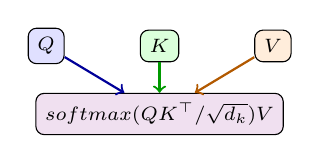
\begin{tikzpicture}[scale=0.72,every node/.style={font=\scriptsize}]
\node[draw,fill=blue!12,rounded corners=3pt] (q) at (0,0) {$Q$};
\node[draw,fill=green!14,rounded corners=3pt] (k) at (2,0) {$K$};
\node[draw,fill=orange!14,rounded corners=3pt] (v) at (4,0) {$V$};
\node[draw,fill=violet!12,rounded corners=3pt] (att) at (2,-1.2) {$\text{softmax}(QK^\top/\sqrt{d_k})V$};
\draw[->,thick,blue!60!black] (q)--(att);
\draw[->,thick,green!60!black] (k)--(att);
\draw[->,thick,orange!70!black] (v)--(att);
\end{tikzpicture}
\caption{Self-attention as $QK^\top$ scoring then value weighting.}
\end{figure}
\begin{example}[Attention scores] For $d_k=64$, $q=[0.2, -0.1,\dots]$, $k=[0.3,0.4,\dots]$, dot $q^\top k\approx 2.1$, scaled $2.1/8=0.26$, softmax over 4 keys gives weights $[0.35,0.28,0.22,0.15]$—soft selection, not hard.
\end{example}

\section{Exercises}
\begin{exercise} Compute $QK^{\top}$ scaling: if $q,k\sim\mathcal{N}(0,1)^{d_k}$, what is $\operatorname{Var}[q^{\top}k]$? Why does $\sqrt{d_k}$ prevent softmax saturation?\end{exercise}
\begin{exercise} Show self-attention is permutation equivariant without PE: if you permute input rows, output permutes identically. Why does this force positional encodings?\end{exercise}
\begin{exercise} Count parameters for one Transformer layer with $d=512$, $h=8$, $d_{\text{ff}}=2048$. Compare to a $3\times3$ conv with same $d$.\end{exercise}
\begin{exercise} Implement causal masking in NumPy self-attention: set scores for $j>i$ to $-\infty$ before softmax. Verify token $i$ only attends to $\le i$.\end{exercise}
\begin{exercise} Contrast BERT (masked LM, bidirectional) and GPT (causal, autoregressive) pre-training. Which suits classification vs generation? Can you convert one to the other?\end{exercise}
% End of Chapter
